\chapter{Marco Te\'{o}rico}

	\section{Antecedentes}
	
		\subsection{Antecedentes de la investigaci\'{o}n}
			
			En el art\'{i}culo cient\'{i}fico titulado \textit{<<Comparing Quantitative Measures of Erythema, Pigmentation and Skin Response using Reflectometry>>}, realizado por \cite{Wagner}, en la Universidad del Estado de Pensilvania, Estados Unidos, y publicado por Pigment Cell Res, se obtiene el \'{i}ndice de eritema, que es utilizado para determinar el nivel inflamatorio de la epidermis de un paciente. El m\'{e}todo utilizado en este art\'{i}culo para su obtenci\'{o}n fue implementado en el nuevo software.
			
			En el art\'{i}culo cient\'{i}fico titulado \textit{<<Recuperaci\'{o}n del Coeficiente de Absorci\'{o}n de la Epidermis en la Piel Humana>>}, realizado por \cite{Narea}, en la Universidad de Carabobo, Venezuela, y publicado por la Sociedad Espa\~{n}ola de \'{O}ptica, se determina el coeficiente de absorci\'{o}n, que es un par\'{a}metro \'{o}ptico asociado a la piel, el cual indica el nivel de concentraci\'{o}n de melanina presente en la epidermis de un paciente. La t\'{e}cnica empleada en dicho art\'{i}culo para calcular este coeficiente fue implementada en el nuevo software.

	\subsection{Observaci\'{o}n directa}
		
			El \textit{<<HunterLab Universal Software>>}, es un software comercial y privativo de 16 bits dise\~{n}ado para el sistema operativo Microsoft Windows versi\'{o}n 3.x, con la posibilidad de ejecutarse en Windows 95, Windows 98, Windows 2000 y Windows XP. Fue creado para la utilizaci\'{o}n del MiniScan XE Plus, adem\'{a}s de otros instrumentos de la empresa HunterLab, y descontinuado en el a\~{n}o 2008. Este software dispone de algunas de las funciones que fueron desarrolladas en el nuevo software, raz\'{o}n por la cual es una referencia importante de observaci\'{o}n. En la figura 2.1 se puede apreciar la vista principal de la interfaz de este software.
			
	\begin{figure}[H]
		\centering
		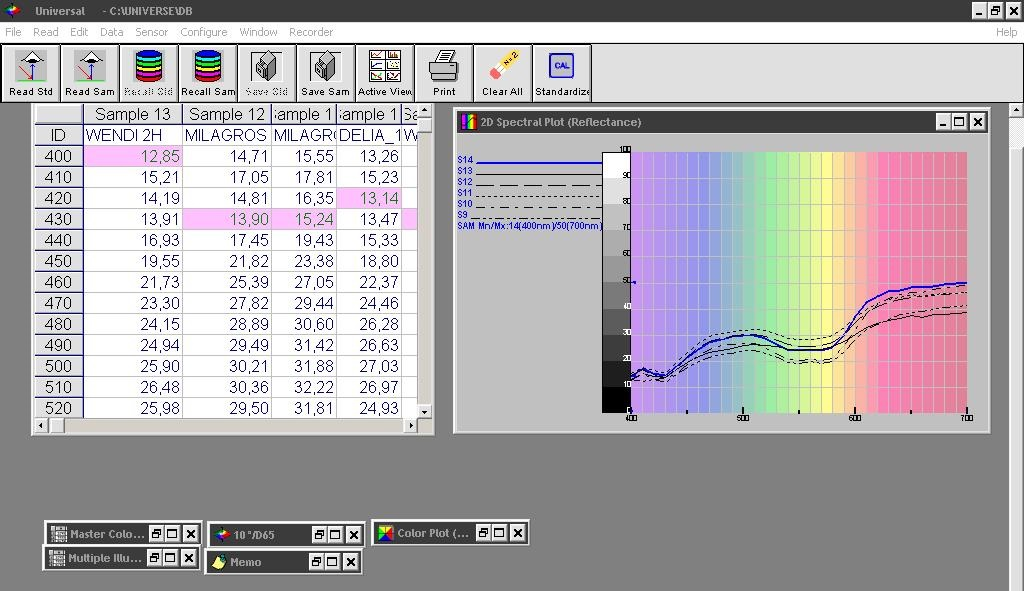
\includegraphics[scale=0.5]{img/universal.jpg}
			\caption[HunterLab Universal Software]{\textit{HunterLab Universal Software} (Fuente: CIMBUC, 2015).}
	\end{figure}

			El archivo denominado \textit{<<MSXE + OCX>>}, es una hoja de c\'{a}lculo habilitada para la ejecuci\'{o}n de macroinstrucciones de Microsoft Excel, que fue proporcionada por el personal de soporte t\'{e}cnico de HunterLab como un ejemplo para utilizar el MiniScan XE Plus, empleando el uso de un kit de control denominado MiniScan XE Plus OCX Kit (MSXE.ocx). Este kit fue dise\~{n}ado por la empresa HunterLab para dar acceso a las caracteristicas comunmente utilizadas por dicho instrumento. El c\'{o}digo contenido en la hoja de c\'{a}lculo se emple\'{o} como referencia para el manejo del kit MSXE.ocx.

	\section{Bases te\'{o}ricas}
	
	\subsection{Espectroscop\'{i}a de reflectancia difusa}
	
		La ERD (espectroscop\'{i}a de reflectancia difusa) es una t\'{e}cnica con la cual se puede estudiar tejido biol\'{o}gico. En el campo de las aplicaciones biom\'{e}dicas resulta \'{u}til para prop\'{o}sitos de diagn\'{o}stico, ya que se pueden estudiar tejidos de manera no invasiva, tambi\'{e}n ha demostrado ser una t\'{e}cnica de gran utilidad en aplicaciones de diagn\'{o}stico en varias situaciones modernas (P\'{e}rez, 2012).
		
		Para llevar a cabo una medici\'{o}n con ERD se requiere hacer incidir la luz de una fuente, cuyo espectro de emisi\'{o}n sea conocido, sobre el tejido que se quiere estudiar. La luz que logra propagarse en el tejido y que es re-emitida por este hacia la superficie irradiada, ser\'{a} capturada por alg\'{u}n dispositivo fotosensible (en el caso de esta investigaci\'{o}n, el MiniScan XE Plus), para ser comparada posteriormente con la luz incidente o espectro de referencia, y as\'{i} poder determinar qu\'{e} tanto cambi\'{o} dicho espectro despu\'{e}s de haber interactuado con el tejido.
		
		Normalmente los datos espectrales de la reflectancia difusa $R(\lambda)$ son multiplicados por un factor de 100 por los dispositivos fotosensibles, para representarlos en forma de curva en una escala del 0\% al 100\%, a lo largo de puntos discretos que representan las longitudes de onda con las que opera dicho dispositivo; tal es el caso del MiniScan XE Plus.
	
	\subsection{Absorbancia aparente}
	
	Seg\'{u}n el \textit{Random House Kernerman Webster's College Dictionary} (2010), el espectro de absorci\'{o}n es la radiaci\'{o}n electromagn\'{e}tica en ciertas longitudes de onda que atraviesa un medio, y que es absorbida por el mismo. En cierto modo, es el opuesto del espectro de reflectancia, es decir, es la luz que no es re-emitida por el tejido en estudio hacia la superficie irradiada, y que aparentemente est\'{a} siendo absorbida por el mismo. 
	
	Por lo tanto, la absorbancia aparente es la luz que est\'{a} siendo absorbida aparentemente por el tejido en estudio, y que no est\'{a} siendo reflejada de vuelta al MiniScan XE Plus. La misma se puede calcular de la siguiente manera: $A(\lambda) = 100 - R(\lambda)$ (recordando que la reflectancia es multiplicada por un factor de 100 por el MiniScan XE Plus) y se puede representar en forma de curva, de la misma manera que la reflectancia difusa.

	\subsection{Iluminante est\'{a}ndar D65}
		
		El tipo de luz bajo el cual se observa un objeto puede afectar su apariencia. Para cuantificar estas fuentes de luz blanca, la \textit{Commission Internationale de l'Eclairage} (CIE) desarroll\'{o} iluminantes est\'{a}ndares para la medici\'{o}n del color.
		\cite{HunterLab} define el iluminante como una tabla cuantificable de n\'{u}meros que representan la energ\'{i}a relativa en comparaci\'{o}n con la longitud de onda de una fuente de luz. 
		
		El iluminante est\'{a}ndar D65, seg\'{u}n es descrito por la \cite{CIE}, tiene el prop\'{o}sito de representar la luz de d\'{i}a promedio, y tiene una temperatura de color correlacionada de aproximadamente 6500 K\degree. Los valores num\'{e}ricos que representan este iluminante se muestran en la tabla 2.1, y su representaci\'{o}n gr\'{a}fica se ilustra en la figura 2.2.

	\subsection{Observador est\'{a}ndar de 10\degree}
	
		\cite{HunterLab-applications} describe que en la observaci\'{o}n visual, el observador es el ojo humano que recibe la luz reflejada desde o a trav\'{e}s de un objeto, y el cerebro el cual percibe la visi\'{o}n. Debido a que los humanos perciben el color y la apariencia de formas distintas, subjetivamente, se han hecho intentos para estandarizar el observador humano como una representaci\'{o}n de lo que una persona promedio ve u observa.
		
		En 1964, se desarroll\'{o} la funci\'{o}n del observador est\'{a}ndar CIE de 10\degree, denominado as\'{i} debido a que los experimentos llevados a cabo para establecer dicho est\'{a}ndar involucraron a sujetos que juzgaban colores, mientras observaban a trav\'{e}s de un agujero que les permit\'{i}a tener un campo de visi\'{o}n de 10\degree. Este observador est\'{a}ndar, en la forma de una funci\'{o}n matem\'{a}tica de la respuesta humana a cada longitud de onda de luz, es utilizado en c\'{a}lculos del color. Los valores num\'{e}ricos de las funciones que representan este est\'{a}ndar se muestran en la tabla 2.2, y su representaci\'{o}n gr\'{a}fica se ilustra en la figura 2.3.
	
	\subsection{Coordenadas de cromaticidad CIE xyz}
	
		La sensaci\'{o}n de luz es producida por radiaci\'{o}n electromagn\'{e}tica visible, que cae dentro de los l\'{i}mites de longitud de onda de 380 nan\'{o}metros y 780 nan\'{o}metros. La radiaci\'{o}n proveniente de la regi\'{o}n de longitud de onda corta produce usualmente la sensaci\'{o}n de luz azul, la radiaci\'{o}n con longitudes de onda entre 520 nan\'{o}metros y 550 nan\'{o}metros son vistas como luz verde, y por encima de alrededor de los 650 nan\'{o}metros se percibe usualmente la luz de color rojo. Estos l\'{i}mites no est\'{a}n bien definidos, y la percepci\'{o}n actual depende fuertemente del estado de adaptaci\'{o}n del ojo y del est\'{i}mulo de luz que rodea el objeto en estudio (Schanda, 2007).
		
		La CIE defini\'{o} un est\'{a}ndar para calcular los valores de estos est\'{i}mulos, denominandolos valores triest\'{i}mulo XYZ o sistema tricrom\'{a}tico CIE XYZ. Tomando en cuenta el rango de longitudes de onda con el que opera el \mbox{MiniScan} XE Plus, estos valores son calculados utilizando las f\'{o}rmulas descritas a continuaci\'{o}n.
		
		$$X = k \int_{400 \text{ nm}}^{700 \text{ nm}} R(\lambda) S(\lambda) \overline{x}(\lambda)d\lambda$$
		
		$$Y = k \int_{400 \text{ nm}}^{700 \text{ nm}} R(\lambda) S(\lambda) \overline{y}(\lambda)d\lambda$$
		
		$$Z = k \int_{400 \text{ nm}}^{700 \text{ nm}} R(\lambda) S(\lambda) \overline{z}(\lambda)d\lambda$$
		
		En donde $R(\lambda)$ es el factor de reflectancia difusa, $S(\lambda)$ es la distribuci\'{o}n de energ\'{i}a espectral relativa de un iluminante est\'{a}ndar, en este caso del iluminante D65 (v\'{e}ase la tabla 2.1), $\overline{x}(\lambda)$, $\overline{y}(\lambda)$ y $\overline{z}(\lambda)$ son las funciones de correspondencia del color, dado el observador est\'{a}ndar CIE de 10\degree (v\'{e}ase la tabla 2.2), y por \'{u}ltimo, $k$ es una constante que se calcula con la f\'{o}rmula mostrada a continuaci\'{o}n.
		
		$$k = \frac{100}{\sum_{\lambda} S(\lambda) \overline{y}(\lambda)d\lambda}$$
		
		De acuerdo con la recomendaci\'{o}n de la CIE, la integraci\'{o}n puede llevarse a cabo con una sumatoria num\'{e}rica a intervalos de longitud de onda, $\bigtriangleup\lambda$, equivalentes a 10 nan\'{o}metros, para el caso del MiniScan XE Plus.
		
		$$X = k \sum_{\lambda} R(\lambda) S(\lambda) \overline{x}(\lambda)\bigtriangleup\lambda$$
		
		$$Y = k \sum_{\lambda} R(\lambda) S(\lambda) \overline{y}(\lambda)\bigtriangleup\lambda$$
		
		$$Z = k \sum_{\lambda} R(\lambda) S(\lambda) \overline{z}(\lambda)\bigtriangleup\lambda$$
		
		Ahora bien, el est\'{i}mulo de un color se puede describir completamente por los tres valores triest\'{i}mulo, pero esta descripci\'{o}n no es muy f\'{a}cilmente concebible. Seg\'{u}n \cite{Schanda}, es dif\'{i}cil imaginar un est\'{i}mulo si solamente se dan sus valores triest\'{i}mulo, y frecuentemente no se buscan los valores absolutos de los mismos. En tales casos se pueden utilizar las coordenadas de cromaticidad xyz. Finalmente, las coordenadas de cromaticidad xyz se definen con las f\'{o}rmulas mostradas a continuaci\'{o}n.
		
		$$x = \frac{X}{X+Y+Z}$$
		
		$$y = \frac{Y}{X+Y+Z}$$
		
		$$z = \frac{Z}{X+Y+Z}$$

	\subsection{Coordenadas del espacio CIELAB}
	
		Seg\'{u}n \cite{Schanda}, los est\'{i}mulos del color son tridimensionales, y la solicitud de extender el espacio del color uniforme a un espacio tridimensional ya hab\'{i}a sido expresada en los a\~{n}os 60. En 1976 se acept\'{o} la recomendaci\'{o}n para el diagrama de espacio del color uniforme CIELAB (L*a*b*).
		
		El espacio del color CIELAB es un sistema para transformar las coordenadas de cromaticidad CIE xyz, a coordenadas L*a*b* representables en un espacio tridimensional, y est\'{a} definido por las ecuaciones descritas a continuaci\'{o}n.
		
		$$L^* = 116f(Y/Y_n) - 16$$
		
		$$a^* = 500[f(X/X_n) - f(Y/Y_n)]$$
		
		$$b^* = 200[f(Y/Y_n) - f(Z/Z_n)]$$
		
		$$\text{Donde } f(X/X_n) = (X/X_n)^{1/3} \text{ si } (X/X_n) > (24/116)^3$$
		$$f(X/X_n) = (841/108)(X/X_n) + 16/116 \text{ si } (X/X_n) \leq (24/116)^3$$
		
		$$\text{Donde } f(Y/Y_n) = (Y/Y_n)^{1/3} \text{ si } (Y/Y_n) > (24/116)^3$$
		$$f(Y/Y_n) = (841/108)(Y/Y_n) + 16/116 \text{ si } (Y/Y_n) \leq (24/116)^3$$
		
		$$\text{Donde } f(Z/Z_n) = (Z/Z_n)^{1/3} \text{ si } (Z/Z_n) > (24/116)^3$$
		$$f(Z/Z_n) = (841/108)(Z/Z_n) + 16/116 \text{ si } (Z/Z_n) \leq (24/116)^3$$
		
		En donde $X$, $Y$, $Z$ son los valores triest\'{i}mulo del color considerado del objeto o tejido en estudio y $X_n$, $Y_n$, $Z_n$ son los valores triest\'{i}mulo de la fuente de luz. Para el caso del iluminante est\'{a}ndar D65, y tomando en cuenta el observador est\'{a}ndar de 10\degree, los valores de $X_n$, $Y_n$, $Z_n$ son $X_n = 94.81$ $Y_n = 100.00$ y $Z_n = 107.32$.

	\subsection{Coeficiente de absorci\'{o}n}
	
		La piel es un medio biol\'{o}gico que se comporta perfectamente como un medio turbio multicapa, donde el principal agente de absorci\'{o}n es la melanina, la cual es producida en la epidermis, y es uno de los par\'{a}metros que determinan la coloraci\'{o}n de la piel (Narea et al., 2015).
		
		En la actualidad, existe el problema de calcular confiablemente los par\'{a}metros \'{o}pticos (entre ellos, el coeficiente de absorci\'{o}n) de los medios turbios a partir del conocimiento de su reflectancia. La determinaci\'{o}n de los par\'{a}metros \'{o}pticos es de vital importancia para el desarrollo de las investigaciones relativas a la caracterizaci\'{o}n de tejidos biol\'{o}gicos, en especial de la piel, empleando m\'{e}todos \'{o}pticos.
		
		\cite{Narea} plantea recuperar el coeficiente de absorci\'{o}n de la epidermis a trav\'{e}s del ajuste trigonom\'{e}trico de los espectros de reflectancia difusa, brindando de esta forma una herramienta matem\'{a}tica que permite relacionar los par\'{a}metros del ajuste de las curvas espectrales con las propiedades \'{o}pticas de la piel.
		
		La f\'{o}rmula empleada para recuperar el coeficiente de absorci\'{o}n de la epidermis, dada una curva espectral $R(\lambda)$, es la mostrada a continuaci\'{o}n.
		
		$$\mu_{a,epi}(a_{0}, \lambda)=Ze^{ka_{0}}6,6 \cdot 10^{11}\lambda^{-3,3}$$
		
		En donde $Z=0,2796$, $k=-7,174$, y $a_{0}$ es un coeficiente hallado aplicando ajuste polinomial por series trigonom\'{e}tricas a la curva espectral $R(\lambda)$.
	
	\subsection{\'{I}ndice de eritema}
	
		Una propiedad fundamental de la piel es su capacidad para responder a la radiaci\'{o}n ultravioleta. En muchas personas y poblaciones estas respuestas son claramente adaptativas, en donde la primera respuesta, el eritema (enrojecimiento), es tanto una se\~{n}al para la persona quemada por el sol de quedarse dentro, como una se\~{n}al de que el sistema inmunol\'{o}gico est\'{a} activo y el proceso de curaci\'{o}n ha comenzado (Wagner et al., 2002). 
		
		La respuesta de la piel result\'{o} ser importante cl\'{i}nicamente cuando los protocolos de tratamiento se establecieron en la d\'{e}cada de los 70 para reg\'{i}menes de fototerapia para la psoriasis y otras enfermedades de la piel. Para calcular el \'{i}ndice de eritema, primero hay que determinar el promedio ponderado de la reflectancia de la luz en el rango de longitud de onda verde, y en el rango de longitud de onda roja, utilizando las f\'{o}rmulas mostradas a continuaci\'{o}n.

		$$R_{verde} = \left.\left.\left[\left(\frac{1}{2}R_{560 \text{ nm}} + R_{570 \text{ nm}} + \frac{1}{2}R_{580 \text{ nm}}\right)\right/2\right]\right/100$$
		
		$$R_{roja} = \left.\left.\left[\left(\frac{1}{2}R_{640 \text{ nm}} + R_{650 \text{ nm}} + R_{660 \text{ nm}} + \frac{1}{2}R_{670 \text{ nm}}\right)\right/3\right]\right/100$$
		
		Teniendo ya el promedio ponderado de dichas reflectancias, la f\'{o}rmula para calcular el \'{i}ndice de eritema es la siguiente.
		
		$$E = 100 \cdot [\log(1/R_{verde}) - \log(1/R_{roja})]$$

\newpage

		\begin{table}[h]
		\small
		\caption[Valores del iluminante D65]{\textit{Valores del iluminante D65} (Fuente: CIE, 2004).}
		\centering
		\setlength{\extrarowheight}{\altocelda}
		\begin{tabulary}{\anchotabla}{|c|c|}
			\hline
			Longitud de onda $\lambda$ & Funci\'{o}n $S(\lambda)$\\ \hline
			400 nm & 82.7549\\ \hline
			410 nm & 91.4860\\ \hline
			420 nm & 93.4318\\ \hline
			430 nm & 86.6823\\ \hline
			440 nm & 104.865\\ \hline
			450 nm & 117.008\\ \hline
			460 nm & 117.812\\ \hline
			470 nm & 114.861\\ \hline
			480 nm & 115.923\\ \hline
			490 nm & 108.811\\ \hline
			500 nm & 109.354\\ \hline
			510 nm & 107.802\\ \hline
			520 nm & 104.790\\ \hline
			530 nm & 107.689\\ \hline
			540 nm & 104.405\\ \hline
			550 nm & 104.046\\ \hline
			560 nm & 100.000\\ \hline
			570 nm & 96.3342\\ \hline
			580 nm & 95.7880\\ \hline
			590 nm & 88.6856\\ \hline
			600 nm & 90.0062\\ \hline
			610 nm & 89.5991\\ \hline
			620 nm & 87.6987\\ \hline
			630 nm & 83.2886\\ \hline
			640 nm & 83.6992\\ \hline
			650 nm & 80.0268\\ \hline
			660 nm & 80.2146\\ \hline
			670 nm & 82.2778\\ \hline
			680 nm & 78.2842\\ \hline
			690 nm & 69.7213\\ \hline
			700 nm & 71.6091\\ \hline
		\end{tabulary}
	\end{table}
	
	\begin{table}[h]
		\small
		\caption[Valores del observador de 10\degree]{\textit{Valores del observador de 10\degree} (Fuente: CIE, 2004).}
		\centering
		\setlength{\extrarowheight}{\altocelda}
		\begin{tabulary}{\anchotabla}{|c|c|c|c|}
			\hline
			Longitud de onda $\lambda$ & Funci\'{o}n $\overline{x}(\lambda)$ & Funci\'{o}n $\overline{y}(\lambda)$ & Funci\'{o}n $\overline{z}(\lambda)$\\ \hline
			400 nm & 0.019110 & 0.002004 & 0.086011\\ \hline
			410 nm & 0.084736 & 0.008756 & 0.389366\\ \hline
			420 nm & 0.204492 & 0.021391 & 0.972542\\ \hline
			430 nm & 0.314679 & 0.038676 & 1.553480\\ \hline
			440 nm & 0.383734 & 0.062077 & 1.967280\\ \hline
			450 nm & 0.370702 & 0.089456 & 1.994800\\ \hline
			460 nm & 0.302273 & 0.128201 & 1.745370\\ \hline
			470 nm & 0.195618 & 0.185190 & 1.317560\\ \hline
			480 nm & 0.080507 & 0.253589 & 0.772125\\ \hline
			490 nm & 0.016172 & 0.339133 & 0.415254\\ \hline
			500 nm & 0.003816 & 0.460777 & 0.218502\\ \hline
			510 nm & 0.037465 & 0.606741 & 0.112044\\ \hline
			520 nm & 0.117749 & 0.761757 & 0.060709\\ \hline
			530 nm & 0.236491 & 0.875211 & 0.030451\\ \hline
			540 nm & 0.376772 & 0.961988 & 0.013676\\ \hline
			550 nm & 0.529826 & 0.991761 & 0.003988\\ \hline
			560 nm & 0.705224 & 0.997340 & 0.000000\\ \hline
			570 nm & 0.705224 & 0.955552 & 0.000000\\ \hline
			580 nm & 1.014160 & 0.868934 & 0.000000\\ \hline
			590 nm & 1.118520 & 0.777405 & 0.000000\\ \hline
			600 nm & 1.123990 & 0.658341 & 0.000000\\ \hline
			610 nm & 1.030480 & 0.527963 & 0.000000\\ \hline
			620 nm & 0.856297 & 0.398057 & 0.000000\\ \hline
			630 nm & 0.647467 & 0.283493 & 0.000000\\ \hline
			640 nm & 0.431567 & 0.179828 & 0.000000\\ \hline
			650 nm & 0.268329 & 0.107633 & 0.000000\\ \hline
			660 nm & 0.152568 & 0.060281 & 0.000000\\ \hline
			670 nm & 0.081261 & 0.031800 & 0.000000\\ \hline
			680 nm & 0.040851 & 0.015905 & 0.000000\\ \hline
			690 nm & 0.019941 & 0.007749 & 0.000000\\ \hline
			700 nm & 0.009577 & 0.003718 & 0.000000\\ \hline
		\end{tabulary}
		
	\end{table}

\FloatBarrier

	\begin{figure}[H]
		\centering
		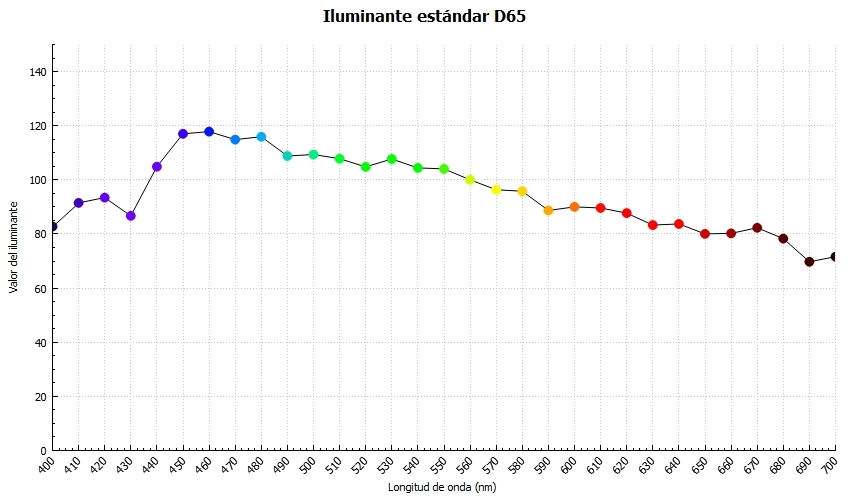
\includegraphics[scale=0.6]{img/curva-iluminante.jpg}
			\caption[Representaci\'{o}n gr\'{a}fica del iluminante est\'{a}ndar D65]{\textit{Representaci\'{o}n gr\'{a}fica del iluminante est\'{a}ndar D65} (Fuente: Autor).}
	\end{figure}
	
	\begin{figure}[H]
		\centering
		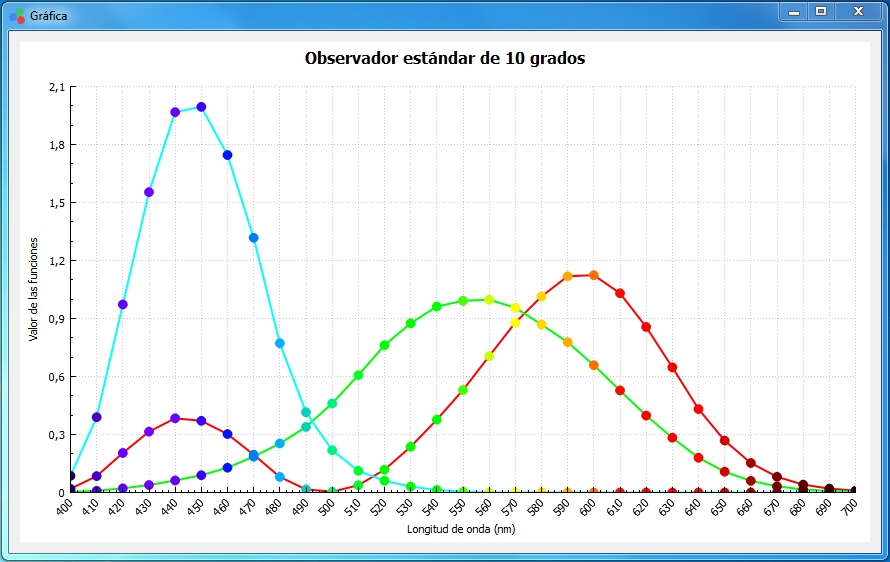
\includegraphics[scale=0.6]{img/curva-observador.jpg}
			\caption[Representaci\'{o}n gr\'{a}fica del observador de 10\degree]{\textit{Representaci\'{o}n gr\'{a}fica del observador de 10\degree. La l\'{i}nea roja representa la funci\'{o}n $\overline{x}(\lambda)$, la l\'{i}nea verde representa la funci\'{o}n $\overline{y}(\lambda)$, y la l\'{i}nea azul representa la funci\'{o}n $\overline{z}(\lambda)$.} (Fuente: Autor).}
	\end{figure}
		